% Options for packages loaded elsewhere
\PassOptionsToPackage{unicode}{hyperref}
\PassOptionsToPackage{hyphens}{url}
\PassOptionsToPackage{dvipsnames,svgnames,x11names}{xcolor}
%
\documentclass[
  letterpaper,
  DIV=11,
  numbers=noendperiod]{scrartcl}

\usepackage{amsmath,amssymb}
\usepackage{lmodern}
\usepackage{iftex}
\ifPDFTeX
  \usepackage[T1]{fontenc}
  \usepackage[utf8]{inputenc}
  \usepackage{textcomp} % provide euro and other symbols
\else % if luatex or xetex
  \usepackage{unicode-math}
  \defaultfontfeatures{Scale=MatchLowercase}
  \defaultfontfeatures[\rmfamily]{Ligatures=TeX,Scale=1}
\fi
% Use upquote if available, for straight quotes in verbatim environments
\IfFileExists{upquote.sty}{\usepackage{upquote}}{}
\IfFileExists{microtype.sty}{% use microtype if available
  \usepackage[]{microtype}
  \UseMicrotypeSet[protrusion]{basicmath} % disable protrusion for tt fonts
}{}
\makeatletter
\@ifundefined{KOMAClassName}{% if non-KOMA class
  \IfFileExists{parskip.sty}{%
    \usepackage{parskip}
  }{% else
    \setlength{\parindent}{0pt}
    \setlength{\parskip}{6pt plus 2pt minus 1pt}}
}{% if KOMA class
  \KOMAoptions{parskip=half}}
\makeatother
\usepackage{xcolor}
\setlength{\emergencystretch}{3em} % prevent overfull lines
\setcounter{secnumdepth}{5}
% Make \paragraph and \subparagraph free-standing
\ifx\paragraph\undefined\else
  \let\oldparagraph\paragraph
  \renewcommand{\paragraph}[1]{\oldparagraph{#1}\mbox{}}
\fi
\ifx\subparagraph\undefined\else
  \let\oldsubparagraph\subparagraph
  \renewcommand{\subparagraph}[1]{\oldsubparagraph{#1}\mbox{}}
\fi


\providecommand{\tightlist}{%
  \setlength{\itemsep}{0pt}\setlength{\parskip}{0pt}}\usepackage{longtable,booktabs,array}
\usepackage{calc} % for calculating minipage widths
% Correct order of tables after \paragraph or \subparagraph
\usepackage{etoolbox}
\makeatletter
\patchcmd\longtable{\par}{\if@noskipsec\mbox{}\fi\par}{}{}
\makeatother
% Allow footnotes in longtable head/foot
\IfFileExists{footnotehyper.sty}{\usepackage{footnotehyper}}{\usepackage{footnote}}
\makesavenoteenv{longtable}
\usepackage{graphicx}
\makeatletter
\def\maxwidth{\ifdim\Gin@nat@width>\linewidth\linewidth\else\Gin@nat@width\fi}
\def\maxheight{\ifdim\Gin@nat@height>\textheight\textheight\else\Gin@nat@height\fi}
\makeatother
% Scale images if necessary, so that they will not overflow the page
% margins by default, and it is still possible to overwrite the defaults
% using explicit options in \includegraphics[width, height, ...]{}
\setkeys{Gin}{width=\maxwidth,height=\maxheight,keepaspectratio}
% Set default figure placement to htbp
\makeatletter
\def\fps@figure{htbp}
\makeatother

\usepackage{booktabs}
\usepackage{longtable}
\usepackage{array}
\usepackage{multirow}
\usepackage{wrapfig}
\usepackage{float}
\usepackage{colortbl}
\usepackage{pdflscape}
\usepackage{tabu}
\usepackage{threeparttable}
\usepackage{threeparttablex}
\usepackage[normalem]{ulem}
\usepackage{makecell}
\usepackage{xcolor}
\KOMAoption{captions}{tableheading}
\makeatletter
\makeatother
\makeatletter
\makeatother
\makeatletter
\@ifpackageloaded{caption}{}{\usepackage{caption}}
\AtBeginDocument{%
\ifdefined\contentsname
  \renewcommand*\contentsname{Table of contents}
\else
  \newcommand\contentsname{Table of contents}
\fi
\ifdefined\listfigurename
  \renewcommand*\listfigurename{List of Figures}
\else
  \newcommand\listfigurename{List of Figures}
\fi
\ifdefined\listtablename
  \renewcommand*\listtablename{List of Tables}
\else
  \newcommand\listtablename{List of Tables}
\fi
\ifdefined\figurename
  \renewcommand*\figurename{Figure}
\else
  \newcommand\figurename{Figure}
\fi
\ifdefined\tablename
  \renewcommand*\tablename{Table}
\else
  \newcommand\tablename{Table}
\fi
}
\@ifpackageloaded{float}{}{\usepackage{float}}
\floatstyle{ruled}
\@ifundefined{c@chapter}{\newfloat{codelisting}{h}{lop}}{\newfloat{codelisting}{h}{lop}[chapter]}
\floatname{codelisting}{Listing}
\newcommand*\listoflistings{\listof{codelisting}{List of Listings}}
\makeatother
\makeatletter
\@ifpackageloaded{caption}{}{\usepackage{caption}}
\@ifpackageloaded{subcaption}{}{\usepackage{subcaption}}
\makeatother
\makeatletter
\@ifpackageloaded{tcolorbox}{}{\usepackage[many]{tcolorbox}}
\makeatother
\makeatletter
\@ifundefined{shadecolor}{\definecolor{shadecolor}{rgb}{.97, .97, .97}}
\makeatother
\makeatletter
\makeatother
\ifLuaTeX
  \usepackage{selnolig}  % disable illegal ligatures
\fi
\IfFileExists{bookmark.sty}{\usepackage{bookmark}}{\usepackage{hyperref}}
\IfFileExists{xurl.sty}{\usepackage{xurl}}{} % add URL line breaks if available
\urlstyle{same} % disable monospaced font for URLs
\hypersetup{
  pdftitle={My title},
  pdfauthor={Myra Li},
  colorlinks=true,
  linkcolor={blue},
  filecolor={Maroon},
  citecolor={Blue},
  urlcolor={Blue},
  pdfcreator={LaTeX via pandoc}}

\title{My title\thanks{Code and data are available at: LINK.}}
\usepackage{etoolbox}
\makeatletter
\providecommand{\subtitle}[1]{% add subtitle to \maketitle
  \apptocmd{\@title}{\par {\large #1 \par}}{}{}
}
\makeatother
\subtitle{My subtitle if needed}
\author{Myra Li}
\date{19 April 2023}

\begin{document}
\maketitle
\begin{abstract}
First sentence. Second sentence. Third sentence. Fourth sentence.
\end{abstract}
\ifdefined\Shaded\renewenvironment{Shaded}{\begin{tcolorbox}[interior hidden, sharp corners, enhanced, frame hidden, breakable, boxrule=0pt, borderline west={3pt}{0pt}{shadecolor}]}{\end{tcolorbox}}\fi

\hypertarget{introduction}{%
\section{Introduction}\label{introduction}}

\hypertarget{sec-data}{%
\section{Data}\label{sec-data}}

\hypertarget{data-source-and-collection}{%
\subsection{Data Source and
Collection}\label{data-source-and-collection}}

\hypertarget{data-cleaning}{%
\subsection{Data Cleaning}\label{data-cleaning}}

\hypertarget{data-visualization}{%
\subsection{Data Visualization}\label{data-visualization}}

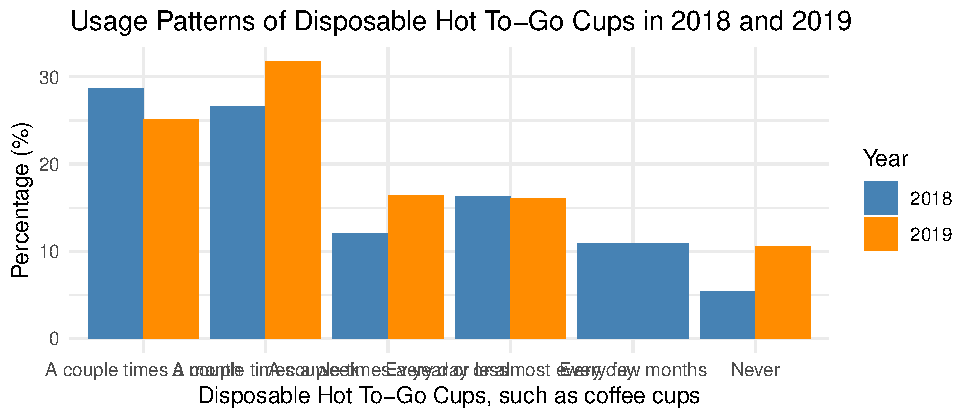
\includegraphics{paper_files/figure-pdf/unnamed-chunk-1-1.pdf}

\hypertarget{model}{%
\section{Model}\label{model}}

Our final logistic regression model is as follows:
\[log(\frac{\hat{p}_i}{\hat{p}_{ref}}) = \beta_{i0} + \beta_{i1}x_{age} + \beta_{i2}x_{gender} + \beta_{i3}x_{education} + \beta_{i4}x_{household_income}+ \beta_{i5}x_{location}\]
The multinomial logistic regression model estimates the probability of a
person's opinion on a by-request/ask-first bylaw aimed at reducing
single-use eating utensil consumption in the City of Toronto. The
possible opinions include: Strongly Support, Somewhat Support, Neither
Support nor Oppose, Somewhat Oppose, Strongly Oppose, and Don't Know.
The model takes into account the following 5 predictor variables:

\begin{enumerate}
\def\labelenumi{\arabic{enumi})}
\item
  Age is a continuous numeric variable representing the individual's
  age.
\item
  Gender is a binary variable (female/male) indicating a person's
  gender.
\item
  Education is a categorical variable representing the highest level of
  education a respondent had at the time of taking the survey.
  Categories include Graduated from college/CEGEP/Trade School,
  Graduated high school, Primary school or less, Some
  college/CEGEP/Trade School, Some high school, Some university but did
  not finish, University graduate degree, and University undergraduate
  degree.
\item
  Household income is a categorical variable indicating the respondent's
  household income range. Categories encompass different income ranges
  and a ``Prefer not to answer'' option.
\item
  Location is a categorical variable representing the respondent's
  location within the City of Toronto. Categories include Toronto, East
  York, Etobicoke, North York, Scarborough, and York.
\end{enumerate}

\hypertarget{results}{%
\section{Results}\label{results}}

\hypertarget{tbl-number}{}
\begin{table}
\caption{\label{tbl-number}Number and Proportion of people opinion on a by-request / ask first
bylaw to reduce the use of single-use eating utensils in the City of
Toronto }\tabularnewline

\centering
\begin{tabular}{l|r|r}
\hline
single\_use\_utensil\_bylaw\_opinion & count & percentage\\
\hline
Don't know & 24 & 2.4\\
\hline
Neither support nor oppose & 114 & 11.4\\
\hline
Somewhat oppose & 62 & 6.2\\
\hline
Somewhat support & 279 & 27.9\\
\hline
Strongly oppose & 45 & 4.5\\
\hline
Strongly support & 476 & 47.6\\
\hline
\end{tabular}
\end{table}

\begin{enumerate}
\def\labelenumi{(\arabic{enumi})}
\tightlist
\item
  presented summarizes the choices made by respondents regarding
  single-use takeaway items. The results indicate that 47.6\% of
  respondents showed strong support for a by-request/ask-first bylaw to
  reduce the use of single-use eating utensils in the City of Toronto.
  Additionally, 27.9\% of respondents somewhat supported the bylaw,
  while 11.4\% of them neither supported nor opposed it. However, 6.2\%
  of respondents somewhat opposed the bylaw, and 4.5\% strongly opposed
  it. These findings suggest that while there is a significant level of
  support for the bylaw, there are still some concerns or reservations
  that need to be addressed.
\end{enumerate}

Overall, the analysis suggests that there is mixed support for the
single-use utensil bylaw, with a slight majority of respondents showing
strong support for it. It is interesting to note that a significant
percentage of respondents are still on the fence, as they neither
support nor oppose the bylaw. This could indicate a lack of awareness or
understanding of the issues surrounding single-use utensils and their
impact on the environment.

\begin{verbatim}
# weights:  246 (200 variable)
initial  value 1791.759469 
iter  10 value 1317.831824
iter  20 value 1250.902050
iter  30 value 1237.797909
iter  40 value 1232.180528
iter  50 value 1229.657429
iter  60 value 1228.928978
iter  70 value 1228.604043
iter  80 value 1228.185006
iter  90 value 1227.752821
iter 100 value 1227.616952
final  value 1227.616952 
stopped after 100 iterations
\end{verbatim}

\hypertarget{discussion}{%
\section{Discussion}\label{discussion}}

\hypertarget{sec-first-point}{%
\subsection{First discussion point}\label{sec-first-point}}

If my paper were 10 pages, then should be be at least 2.5 pages. The
discussion is a chance to show off what you know and what you learnt
from all this.

\hypertarget{second-discussion-point}{%
\subsection{Second discussion point}\label{second-discussion-point}}

\hypertarget{third-discussion-point}{%
\subsection{Third discussion point}\label{third-discussion-point}}

\hypertarget{weaknesses-and-next-steps}{%
\subsection{Weaknesses and next steps}\label{weaknesses-and-next-steps}}

Weaknesses and next steps should also be included.

\newpage

\appendix

\hypertarget{appendix}{%
\section*{Appendix}\label{appendix}}
\addcontentsline{toc}{section}{Appendix}

\hypertarget{additional-data-details}{%
\section{Additional data details}\label{additional-data-details}}

\hypertarget{sec-model-details}{%
\section{Model details}\label{sec-model-details}}

\hypertarget{posterior-predictive-check}{%
\subsection{Posterior predictive
check}\label{posterior-predictive-check}}

In we implement a posterior predictive check. This shows\ldots{}

In we compare the posterior with the prior. This shows\ldots{}

\hypertarget{diagnostics}{%
\subsection{Diagnostics}\label{diagnostics}}

is a trace plot. It shows\ldots{} This suggests\ldots{}

is a Rhat plot. It shows\ldots{} This suggests\ldots{}

\newpage

\hypertarget{references}{%
\section{References}\label{references}}



\end{document}
